\documentclass[11pt,a4paper]{article}
\usepackage[utf8]{inputenc}
\usepackage[margin=0.8in]{geometry}
\usepackage{tikz}
\usetikzlibrary{shapes.geometric, arrows, positioning, calc, fit, backgrounds}
\usepackage{xcolor}
\usepackage{hyperref}
\usepackage{listings}
\usepackage{enumitem}
\usepackage{tcolorbox}
\usepackage{graphicx}
\usepackage{tabularx}
\usepackage{booktabs}

% Code listing setup
\lstset{
    language=Java,
    basicstyle=\ttfamily\small,
    keywordstyle=\color{blue}\bfseries,
    commentstyle=\color{green!50!black},
    stringstyle=\color{red!70!black},
    numbers=left,
    numberstyle=\tiny\color{gray},
    numbersep=5pt,
    frame=single,
    breaklines=true,
    breakatwhitespace=true,
    tabsize=4,
    showstringspaces=false,
    captionpos=b
}

% Define colors
\definecolor{startcolor}{RGB}{76, 175, 80}
\definecolor{endcolor}{RGB}{244, 67, 54}
\definecolor{processcolor}{RGB}{33, 150, 243}
\definecolor{decisioncolor}{RGB}{255, 193, 7}
\definecolor{actioncolor}{RGB}{156, 39, 176}
\definecolor{issuecolor}{RGB}{255, 87, 34}
\definecolor{fixedcolor}{RGB}{76, 175, 80}
\definecolor{warningcolor}{RGB}{255, 152, 0}
\definecolor{infocolor}{RGB}{3, 169, 244}

% TikZ styles - IMPROVED to match flowchart document
\tikzstyle{startstop} = [rectangle, rounded corners, minimum width=3cm, minimum height=1cm, text centered, draw=black, fill=startcolor!30, align=center]
\tikzstyle{process} = [rectangle, minimum width=3cm, minimum height=1cm, text centered, draw=black, fill=processcolor!30, align=center]
\tikzstyle{decision} = [diamond, minimum width=3.5cm, minimum height=1.2cm, text centered, draw=black, fill=decisioncolor!30, aspect=3, align=center, text width=2.5cm]
\tikzstyle{action} = [rectangle, rounded corners, minimum width=3cm, minimum height=1cm, text centered, draw=black, fill=actioncolor!30, align=center]
\tikzstyle{arrow} = [thick,->,>=stealth, rounded corners]
\tikzstyle{state} = [rectangle, rounded corners, minimum width=3cm, minimum height=1cm, text centered, draw=black, fill=blue!20, align=center, text width=3cm]
\tikzstyle{hardware} = [rectangle, rounded corners, minimum width=3cm, minimum height=1cm, text centered, draw=black, fill=orange!20, align=center]
\tikzstyle{sensor} = [ellipse, minimum width=2.5cm, minimum height=0.8cm, text centered, draw=black, fill=green!20, align=center]
\tikzstyle{motor} = [rectangle, minimum width=2.5cm, minimum height=0.8cm, text centered, draw=black, fill=red!20, align=center]

\title{\textbf{Quanta Programming Guide}\\FTC Robot Programming Fundamentals\\Team Knowledge Transfer Document}
\author{Quanta FTC Programming Team}
\date{January 2026 Season}

\begin{document}

\maketitle
\tableofcontents
\newpage

% ============================================================================
\section{Introduction}
% ============================================================================

This document serves as a comprehensive guide for Quanta programming team members. It covers all the fundamental concepts needed to understand and contribute to our robot's software.

\begin{tcolorbox}[colback=infocolor!10, colframe=infocolor, title=What You'll Learn]
\begin{enumerate}
    \item \textbf{Hardware Architecture} - Controllers, sensors, and actuators
    \item \textbf{Motor Control} - Different modes and when to use them
    \item \textbf{State Machines (FSM)} - How we track robot state intelligently
    \item \textbf{OpModes} - Manual and autonomous programs explained
\end{enumerate}
\end{tcolorbox}

\newpage
% ============================================================================
\section{Hardware Architecture: Controllers}
% ============================================================================

\subsection{REV Control Hub}

The \textbf{REV Control Hub} is the brain of our robot. It runs the Robot Controller app and directly interfaces with motors, servos, and sensors.

\begin{tcolorbox}[colback=processcolor!10, colframe=processcolor, title=REV Control Hub Features]
\begin{itemize}
    \item Built-in \textbf{IMU} (Inertial Measurement Unit) - Provides yaw, pitch, roll
    \item 4 DC Motor ports (with encoders)
    \item 6 Servo ports (PWM signals)
    \item 4 Analog input ports
    \item 8 Digital I/O ports
    \item I2C bus for sensors
    \item USB ports for cameras
    \item WiFi for Driver Station communication
\end{itemize}
\end{tcolorbox}

\subsection{REV Expansion Hub}

When we need more ports than the Control Hub provides, we add an \textbf{Expansion Hub}:
\begin{itemize}
    \item Additional 4 DC Motor ports
    \item Additional 6 Servo ports
    \item More sensor ports
    \item Connected to Control Hub via RS-485 cable
\end{itemize}

\subsection{Port Types and Signal Types}

\begin{center}
\begin{tabular}{|l|c|l|l|}
\hline
\textbf{Port Type} & \textbf{Count} & \textbf{Signal Type} & \textbf{Used For} \\
\hline
Motor Port & 4 per hub & PWM + Encoder & DC Motors \\
Servo Port & 6 per hub & PWM (0-180°) & Servos \\
Analog Input & 4 & 0-3.3V analog & Potentiometers \\
Digital I/O & 8 & 0V / 3.3V & Limit switches, LEDs \\
I2C & 4 buses & I2C protocol & Color sensors, IMU \\
USB & varies & USB 2.0 & Cameras \\
\hline
\end{tabular}
\end{center}

\newpage
\subsection{Hardware Connection Diagram}

\begin{center}
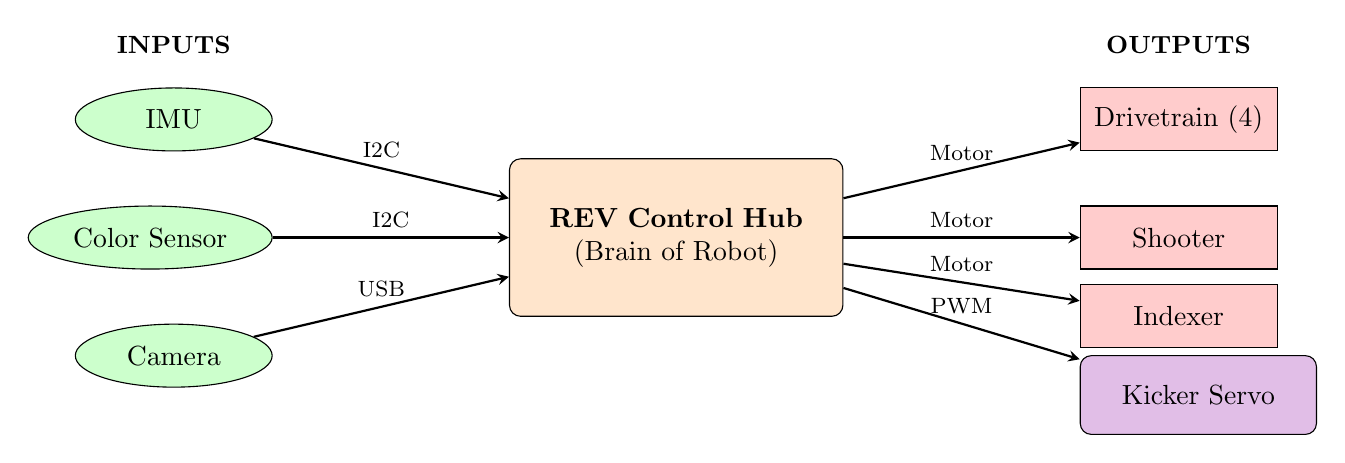
\begin{tikzpicture}[node distance=1.5cm, auto]

% Control Hub in center
\node (hub) [hardware, text width=4cm, minimum height=2cm] {\textbf{REV Control Hub}\\(Brain of Robot)};

% Sensors on the left
\node (imu) [sensor, left=3cm of hub, yshift=1.5cm] {IMU};
\node (color) [sensor, left=3cm of hub, yshift=0cm] {Color Sensor};
\node (camera) [sensor, left=3cm of hub, yshift=-1.5cm] {Camera};

% Motors on the right
\node (drive) [motor, right=3cm of hub, yshift=1.5cm] {Drivetrain (4)};
\node (shooter) [motor, right=3cm of hub, yshift=0cm] {Shooter};
\node (indexer) [motor, right=3cm of hub, yshift=-1cm] {Indexer};
\node (kicker) [action, right=3cm of hub, yshift=-2cm] {Kicker Servo};

% Arrows from sensors to hub
\draw [arrow] (imu) -- node[above, font=\footnotesize] {I2C} (hub);
\draw [arrow] (color) -- node[above, font=\footnotesize] {I2C} (hub);
\draw [arrow] (camera) -- node[above, font=\footnotesize] {USB} (hub);

% Arrows from hub to motors
\draw [arrow] (hub) -- node[above, font=\footnotesize] {Motor} (drive);
\draw [arrow] (hub) -- node[above, font=\footnotesize] {Motor} (shooter);
\draw [arrow] (hub) -- node[above, font=\footnotesize] {Motor} (indexer);
\draw [arrow] (hub) -- node[above, font=\footnotesize] {PWM} (kicker);

% Labels
\node[above=0.3cm of imu, font=\small\bfseries] {INPUTS};
\node[above=0.3cm of drive, font=\small\bfseries] {OUTPUTS};

\end{tikzpicture}
\end{center}

\newpage
% ============================================================================
\section{Sensors: Robot Inputs}
% ============================================================================

Sensors are how the robot "sees" and "feels" the world. They provide input data for decision-making.

\subsection{IMU (Inertial Measurement Unit)}

The IMU is embedded in the Control Hub and measures robot orientation.

\begin{tcolorbox}[colback=fixedcolor!10, colframe=fixedcolor, title=What IMU Measures]
\begin{itemize}
    \item \textbf{Yaw} - Rotation around vertical axis (heading)
    \item \textbf{Pitch} - Tilt forward/backward
    \item \textbf{Roll} - Tilt left/right
    \item \textbf{Acceleration} - Movement in X, Y, Z directions
\end{itemize}
\end{tcolorbox}

\textbf{Our Usage:} Field-centric driving uses the yaw angle to rotate joystick inputs to match field orientation.

\begin{lstlisting}[caption={IMU Initialization from A1.java}]
// Initialize IMU
imu = hardwareMap.get(IMU.class, "imu");
IMU.Parameters parameters = new IMU.Parameters(
    new RevHubOrientationOnRobot(
        RevHubOrientationOnRobot.LogoFacingDirection.UP,
        RevHubOrientationOnRobot.UsbFacingDirection.FORWARD
    )
);
imu.initialize(parameters);
\end{lstlisting}

\begin{lstlisting}[caption={Using IMU for Field-Centric Drive}]
// Get robot heading (yaw)
YawPitchRollAngles botAngles = imu.getRobotYawPitchRollAngles();
double botHeading = -botAngles.getYaw(AngleUnit.RADIANS);

// Transform joystick inputs to field-centric
double rotX = x * Math.cos(botHeading) - y * Math.sin(botHeading);
double rotY = x * Math.sin(botHeading) + y * Math.cos(botHeading);
\end{lstlisting}

\newpage
\subsection{Color Sensor (RevColorSensorV3)}

We use the REV Color Sensor V3 to detect colored balls (artifacts).

\begin{tcolorbox}[colback=actioncolor!10, colframe=actioncolor, title=Color Sensor Capabilities]
\begin{itemize}
    \item \textbf{RGB Values} - Red, Green, Blue light intensity (0-65535)
    \item \textbf{Distance} - Proximity detection in cm
    \item \textbf{I2C Interface} - Connected via I2C port
\end{itemize}
\end{tcolorbox}

\begin{lstlisting}[caption={Color Sensor Reading from RevolverSubsystem.java}]
// Read sensor values
double distance = sensor.getDistance(DistanceUnit.CM);
int r = sensor.red();
int g = sensor.green();
int b = sensor.blue();

// Determine ball color
SlotColor detected = determineColor(distance, r, g, b);
\end{lstlisting}

\subsection{Color Detection Logic}

\begin{center}
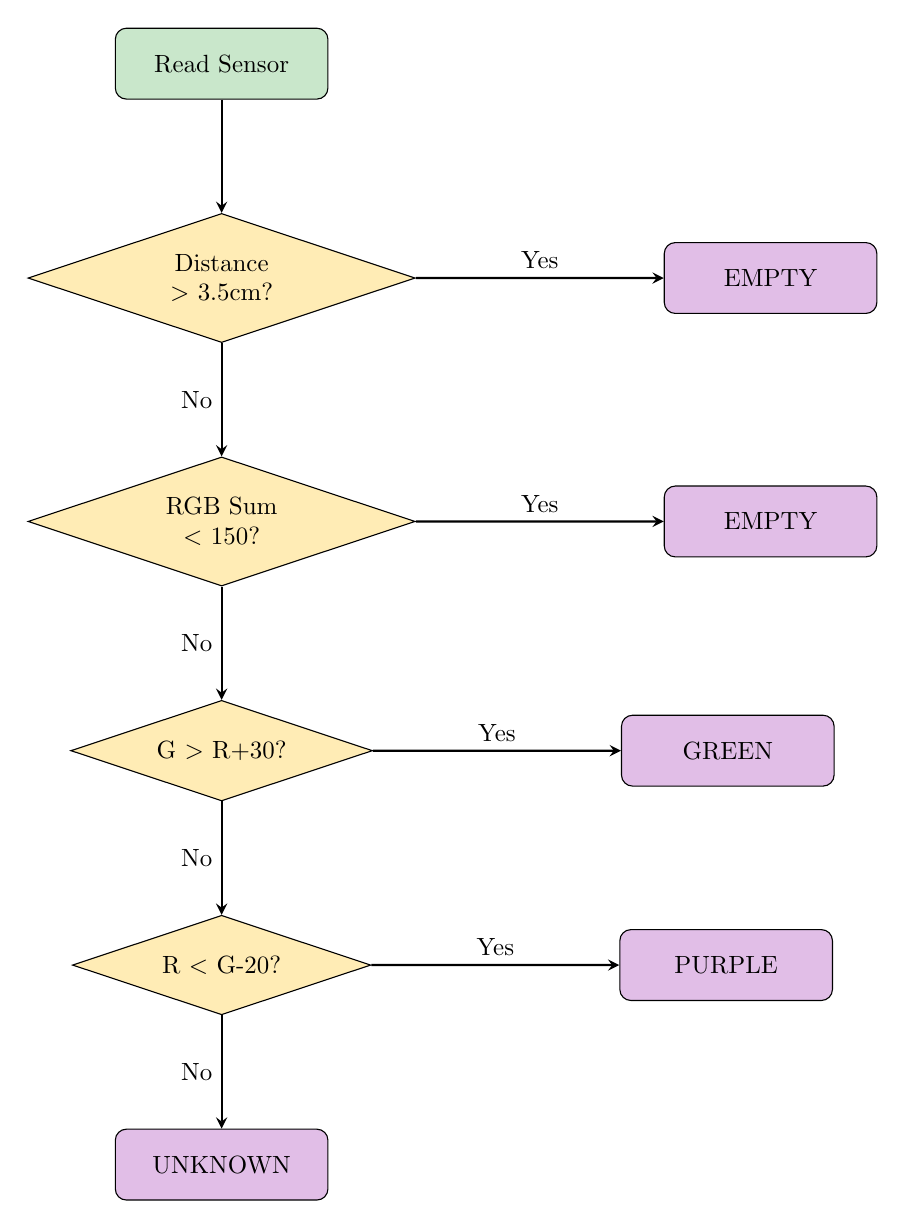
\begin{tikzpicture}[node distance=1.6cm, auto, scale=0.9, transform shape]

% Vertical spine
\node (read) [startstop] {Read Sensor};
\node (dist) [decision, below=of read] {Distance $>$ 3.5cm?};
\node (bright) [decision, below=of dist] {RGB Sum $<$ 150?};
\node (green) [decision, below=of bright] {G $>$ R+30?};
\node (purple) [decision, below=of green] {R $<$ G-20?};
\node (unknown) [action, below=of purple] {UNKNOWN};

% Results on right - spaced to avoid overlap
\node (empty1) [action, right=3.5cm of dist] {EMPTY};
\node (empty2) [action, right=3.5cm of bright] {EMPTY};
\node (gret) [action, right=3.5cm of green] {GREEN};
\node (pret) [action, right=3.5cm of purple] {PURPLE};

% Arrows
\draw [arrow] (read) -- (dist);
\draw [arrow] (dist) -- node[above] {Yes} (empty1);
\draw [arrow] (dist) -- node[left] {No} (bright);
\draw [arrow] (bright) -- node[above] {Yes} (empty2);
\draw [arrow] (bright) -- node[left] {No} (green);
\draw [arrow] (green) -- node[above] {Yes} (gret);
\draw [arrow] (green) -- node[left] {No} (purple);
\draw [arrow] (purple) -- node[above] {Yes} (pret);
\draw [arrow] (purple) -- node[left] {No} (unknown);

\end{tikzpicture}
\end{center}

\newpage
% ============================================================================
\section{Actuators: Motors and Servos}
% ============================================================================

Actuators are outputs that make the robot move and perform actions.

\subsection{Motor Types We Use}

\begin{center}
\begin{tabular}{|l|l|l|l|}
\hline
\textbf{Motor Type} & \textbf{Used For} & \textbf{Gear Ratio} & \textbf{Encoder} \\
\hline
HD Hex DC Motor & Drivetrain, Shooter & 20:1 typical & 28 ticks/rev \\
Core Hex DC Motor & Intake, Indexer & 40:1, 72:1 & 28 ticks/rev \\
\hline
\end{tabular}
\end{center}

\subsection{REV Motor Encoders}

REV motors have built-in \textbf{quadrature encoders} that track rotation.

\begin{tcolorbox}[colback=warningcolor!10, colframe=warningcolor, title=Understanding Ticks]
\begin{itemize}
    \item Encoders produce "ticks" - pulses per motor rotation
    \item REV motors: 28 ticks per motor shaft revolution
    \item With gearbox: \texttt{ticks = 28 × gear\_ratio}
    \item Example: 20:1 HD Hex = 28 × 20 = 560 ticks/output revolution
\end{itemize}
\end{tcolorbox}

\subsection{Servo (Kicker)}

Servos are position-controlled motors used for precise angular movement.

\begin{lstlisting}[caption={Servo Control for Kicker}]
// Servo positions (0.0 to 1.0)
private static final double KICKER_RETRACT = 0.3;
private static final double KICKER_EJECT = 0.8;

// Set servo position
kicker.setPosition(KICKER_EJECT);  // Servo moves to 80% position
\end{lstlisting}

\newpage
\subsection{DC Motor Control: Power vs Velocity}

There are two fundamentally different ways to control DC motors:

\subsubsection{Method 1: Raw Power Control}

\begin{lstlisting}[caption={Raw Power Control}]
motor.setPower(0.5);  // 50% power
\end{lstlisting}

\begin{itemize}
    \item Value: -1.0 to +1.0 (percentage of battery voltage)
    \item Simple but imprecise
    \item Speed varies with battery level and load
    \item Used for: Intake, simple mechanisms
\end{itemize}

\subsubsection{Method 2: Velocity Control}

\begin{lstlisting}[caption={Velocity Control}]
motor.setVelocity(2000);  // 2000 ticks per second
\end{lstlisting}

\begin{itemize}
    \item Value: ticks per second
    \item Uses PID controller to maintain constant speed
    \item Consistent regardless of battery/load
    \item Used for: Shooter, precision mechanisms
\end{itemize}

\begin{tcolorbox}[colback=issuecolor!10, colframe=issuecolor, title=Warning: Don't Mix Both!]
If you call both \texttt{setVelocity()} and \texttt{setPower()} on the same motor, the velocity controller takes priority. This caused our shooter power issue - the velocity PID always drove to max speed regardless of the power setting.
\end{tcolorbox}

\newpage
\subsection{DC Motor Run Modes}

The FTC SDK provides different motor run modes:

\begin{center}
\begin{tabular}{|l|p{8cm}|}
\hline
\textbf{Mode} & \textbf{Description} \\
\hline
\texttt{RUN\_WITHOUT\_ENCODER} & Simple power control. Encoder not used. Best for intake motors. \\
\hline
\texttt{RUN\_USING\_ENCODER} & Velocity control with PID. Motor maintains constant speed. Best for shooter. \\
\hline
\texttt{RUN\_TO\_POSITION} & Position control. Motor moves to target tick count and holds. Best for indexer. \\
\hline
\texttt{STOP\_AND\_RESET\_ENCODER} & Resets encoder count to zero. Call before setting target position. \\
\hline
\end{tabular}
\end{center}

\begin{lstlisting}[caption={Motor Mode Setup from RevolverSubsystem.java}]
// Indexer: Position control (RUN_TO_POSITION)
indexer.setDirection(DcMotorSimple.Direction.REVERSE);
indexer.setMode(DcMotor.RunMode.STOP_AND_RESET_ENCODER);  // Reset to 0
indexer.setTargetPosition(0);
indexer.setMode(DcMotor.RunMode.RUN_TO_POSITION);         // Enable position control
indexer.setZeroPowerBehavior(DcMotor.ZeroPowerBehavior.BRAKE);
indexer.setVelocityPIDFCoefficients(40, 5, 5, 10);        // Custom PID

// Intake: Simple power control (no encoder feedback)
intake.setMode(DcMotor.RunMode.RUN_WITHOUT_ENCODER);

// Shooter: Velocity control for consistent speed
shooter.setMode(DcMotor.RunMode.RUN_USING_ENCODER);
\end{lstlisting}

\subsection{Zero Power Behavior}

What happens when motor power is set to 0:

\begin{center}
\begin{tabular}{|l|l|}
\hline
\textbf{Mode} & \textbf{Behavior} \\
\hline
\texttt{BRAKE} & Motor actively resists movement (short-circuit braking) \\
\texttt{FLOAT} & Motor coasts freely (no resistance) \\
\hline
\end{tabular}
\end{center}

\textbf{Our Usage:} All drivetrain motors use \texttt{BRAKE} for precise stopping.

\newpage
% ============================================================================
\section{Finite State Machines (FSM)}
% ============================================================================

\subsection{What is a State Machine?}

A Finite State Machine is a way to organize code where the robot can only be in \textbf{one state at a time}, and transitions between states based on conditions.

\begin{tcolorbox}[colback=infocolor!10, colframe=infocolor, title=FSM Benefits]
\begin{itemize}
    \item \textbf{Predictable:} Robot behavior is well-defined for each state
    \item \textbf{Debuggable:} Easy to see which state robot is in
    \item \textbf{Intelligent:} Robot tracks its own status automatically
    \item \textbf{Safe:} Prevents conflicting actions
\end{itemize}
\end{tcolorbox}

\subsection{RevolverSubsystem State Machine}

Our revolver system uses a state machine to manage ball loading and shooting:

\begin{lstlisting}[caption={State Enumeration from RevolverSubsystem.java}]
public enum RevolverState {
    LOADING,           // Aligning EMPTY slot to Intake (0 deg)
    INDEXING,          // Moving to next EMPTY slot
    WAIT_FOR_INTAKE_CLEAR,  // Wait for ball to clear
    SHOOTING_ALIGN,    // Rotating color slot to Shooter (240 deg)
    READY_TO_SHOOT,    // Aligned, waiting for trigger
    SHOOTING,          // Kicker sequence active
    FULL               // All slots full
}
\end{lstlisting}

\newpage
\subsection{RevolverSubsystem State Diagram}

\begin{center}
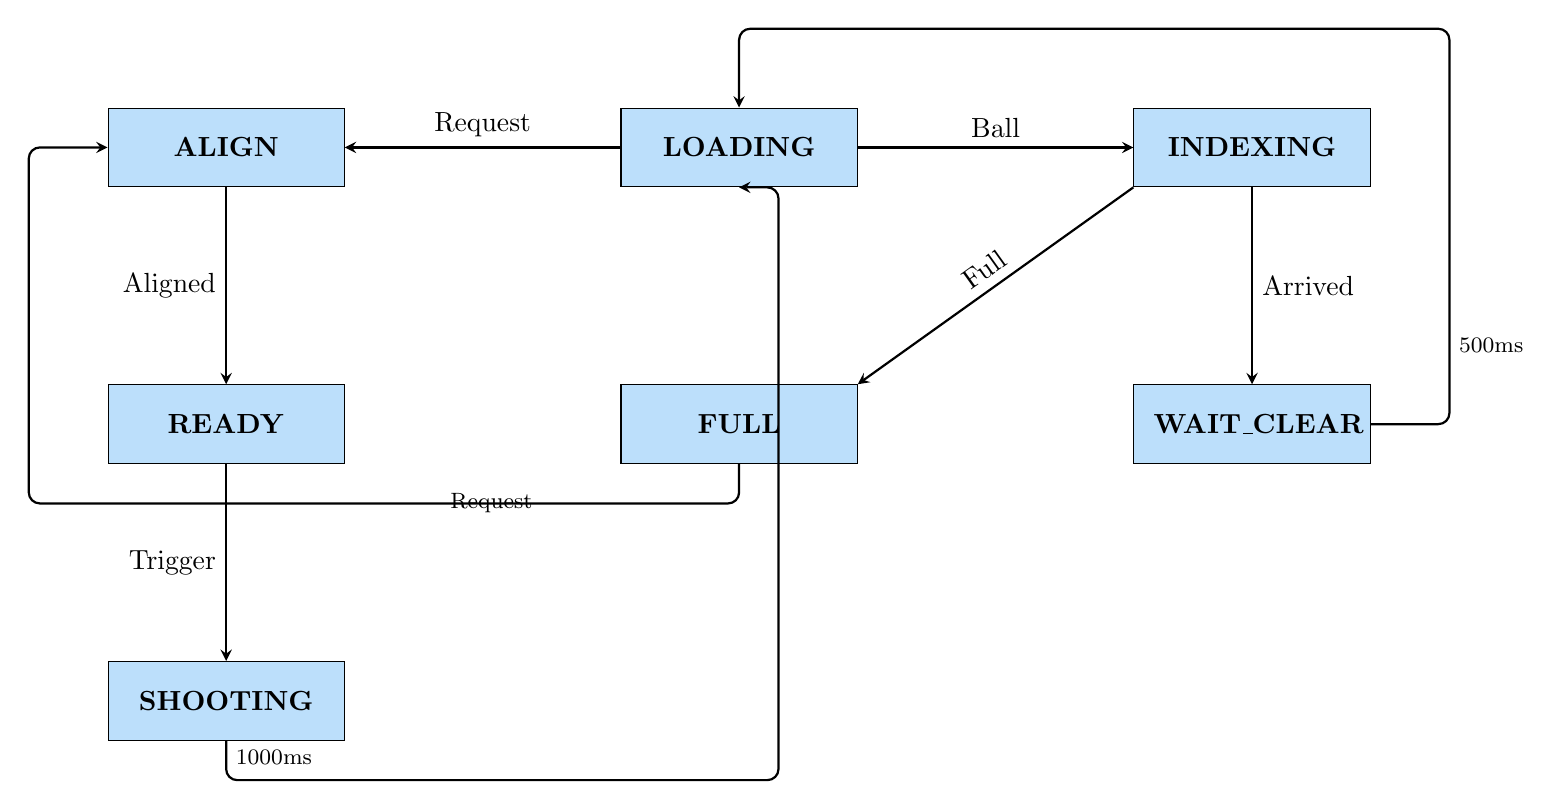
\begin{tikzpicture}[node distance=2.5cm, auto]

% Center node
\node (loading) [process, text width=2.5cm] {\textbf{LOADING}};

% Right Column (Intake path)
\node (indexing) [process, right=3.5cm of loading, text width=2.5cm] {\textbf{INDEXING}};
\node (wait) [process, below=of indexing, text width=2.5cm] {\textbf{WAIT\_CLEAR}};

% Center Bottom
\node (full) [process, below=of loading, text width=2.5cm] {\textbf{FULL}};

% Left Column (Shooting path)
\node (align) [process, left=3.5cm of loading, text width=2.5cm] {\textbf{ALIGN}};
\node (ready) [process, below=of align, text width=2.5cm] {\textbf{READY}};
\node (shooting) [process, below=of ready, text width=2.5cm] {\textbf{SHOOTING}};

% --- Transitions with Explicit Routing ---

% 1. Loading -> Indexing (Straight)
\draw [arrow] (loading) -- node[above] {Ball} (indexing);

% 2. Indexing -> Wait (Straight Down)
\draw [arrow] (indexing) -- node[right] {Arrived} (wait);

% 3. Wait -> Loading (Wide path above)
\draw [arrow] (wait.east) -- ++(1,0) |- ([yshift=1cm]loading.north) -- (loading.north);
\node [right, font=\footnotesize] at ($(wait.east)+(1,1)$) {500ms};

% 4. Indexing -> Full (Diagonal)
\draw [arrow] (indexing.south west) -- node[sloped, above] {Full} (full.north east);

% 5. Loading -> Align (Straight)
\draw [arrow] (loading) -- node[above] {Request} (align);

% 6. Full -> Align (Wide path below and left)
\draw [arrow] (full.south) -- ++(0,-0.5) -| ([xshift=-1cm]align.west) -- (align.west);
\node [left, font=\footnotesize] at ($(full.south)+(-2.5,-0.5)$) {Request};

% 7. Align -> Ready (Straight Down)
\draw [arrow] (align) -- node[left] {Aligned} (ready);

% 8. Ready -> Shooting (Straight Down)
\draw [arrow] (ready) -- node[left] {Trigger} (shooting);

% 9. Shooting -> Loading (Wide path below and right)
\draw [arrow] (shooting.south) -- ++(0,-0.5) -| ([xshift=0.5cm]loading.south) -- (loading.south);
\node [below right, font=\footnotesize] at (shooting.south) {1000ms};

\end{tikzpicture}
\end{center}

\subsection{State Machine Update Loop}

The state machine runs in the \texttt{update()} method called every loop:

\begin{lstlisting}[caption={State Machine Pattern}]
public void update() {
    // 1. Read sensors
    SlotColor detected = readColorNow();
    
    // 2. State machine switch
    switch (currentState) {
        case LOADING:
            // Actions for LOADING state
            if (detected != SlotColor.EMPTY) {
                currentState = RevolverState.INDEXING;  // Transition
            }
            break;
            
        case INDEXING:
            // Actions for INDEXING state
            if (isIndexerAtTarget()) {
                currentState = RevolverState.WAIT_FOR_INTAKE_CLEAR;
            }
            break;
        // ... more states
    }
}
\end{lstlisting}

\newpage
% ============================================================================
\section{OpModes Explained}
% ============================================================================

\subsection{OpMode Types}

\begin{center}
\begin{tabular}{|l|l|l|}
\hline
\textbf{Type} & \textbf{Parent Class} & \textbf{Used For} \\
\hline
TeleOp & \texttt{OpMode} or \texttt{LinearOpMode} & Driver-controlled period \\
Autonomous & \texttt{LinearOpMode} & 30-second autonomous period \\
\hline
\end{tabular}
\end{center}

\begin{itemize}
    \item \texttt{OpMode} - Loop-based, \texttt{loop()} called repeatedly
    \item \texttt{LinearOpMode} - Sequential, runs top to bottom with \texttt{sleep()}
\end{itemize}

\subsection{A1 - Basic Manual TeleOp}

Location: \texttt{TeamCode/.../opmodes/A1.java}

\textbf{Purpose:} Simple manual control with field-centric driving and SimpleRevolver.

\begin{lstlisting}[caption={A1 Control Mapping}]
// Controls:
// RT/LT      - Intake forward/reverse
// Circle    - Toggle shooter on/off
// Cross     - Manual index next slot
// LB        - Kick (timer-based)
// D-pad     - Manual trim +/- 5 ticks
// RB        - Slow mode (30% speed)
// Options   - Reset IMU heading
\end{lstlisting}

\textbf{Key Features:}
\begin{itemize}
    \item Uses \texttt{SimpleRevolver} subsystem
    \item Field-centric mecanum drive with IMU
    \item Timer-based kicker sequence (500ms spool, 600ms eject, 600ms retract)
    \item All manual control - no auto-indexing
\end{itemize}

\newpage
\subsection{A3 - Smart Indexing TeleOp}

Location: \texttt{TeamCode/.../opmodes/A3.java}

\textbf{Purpose:} Enhanced TeleOp with automatic ball detection and indexing.

\begin{lstlisting}[caption={A3 Auto-Indexing Logic}]
// AUTO-INDEXING: Detect ball during intake
if (intaking) {
    SlotColor currentColor = revolver.readColorNow();
    boolean ballDetected = (currentColor == SlotColor.GREEN ||
                           currentColor == SlotColor.PURPLE);
    
    // Edge detection: ball just entered?
    boolean justDetected = ballDetected && 
                          (lastDetectedColor == SlotColor.EMPTY);
    
    // Auto-index with cooldown to prevent double-triggering
    if (justDetected && (currentTime - lastIndexTime > 800)) {
        revolver.indexerNextSlot();  // Automatic rotation!
        lastIndexTime = currentTime;
    }
    lastDetectedColor = currentColor;
}
\end{lstlisting}

\textbf{Key Differences from A1:}
\begin{itemize}
    \item Uses \texttt{RevolverSubsystem} (more advanced) instead of SimpleRevolver
    \item \textbf{Auto-indexing} when ball detected during intake
    \item Direct kicker control (bypasses FSM) with \texttt{disableFSMKickerControl = true}
    \item Edge detection prevents double-indexing same ball
    \item 800ms cooldown between auto-indexes
\end{itemize}

\begin{lstlisting}[caption={A3 Direct Kicker Control (bypasses FSM)}]
// CRITICAL: Disable FSM kicker control in init()
revolver.disableFSMKickerControl = true;

// Direct timer-based kicker (like SimpleRevolver)
if (isKicking) {
    long elapsed = System.currentTimeMillis() - kickTimer;
    if (elapsed < 500) {
        revolver.kicker.setPosition(KICKER_RETRACT);  // Spool up
    } else if (elapsed < 1100) {
        revolver.kicker.setPosition(KICKER_EJECT);    // Kick!
    } else if (elapsed < 1700) {
        revolver.kicker.setPosition(KICKER_RETRACT);  // Retract
    } else {
        isKicking = false;  // Done
    }
}
\end{lstlisting}

\newpage
\subsection{DecodeShootingAuto - Autonomous Mode}

Location: \texttt{TeamCode/.../DecodeAuto/DecodeShootingAuto.java}

\textbf{Purpose:} Full autonomous sequence with AprilTag detection and artifact collection.

\subsubsection{Autonomous Flow Overview}

\begin{center}
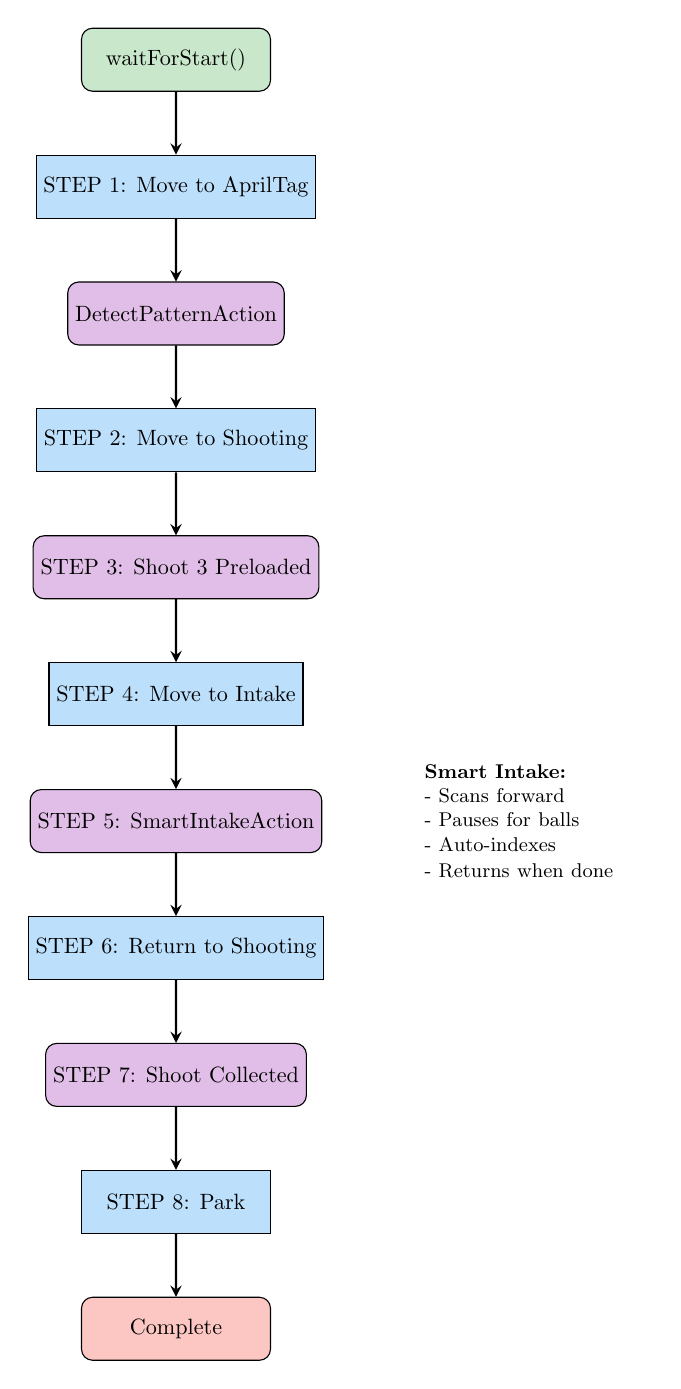
\begin{tikzpicture}[node distance=1cm, scale=0.8, transform shape]

% Nodes - vertical flow
\node (start) [startstop] {waitForStart()};
\node (step1) [process, below=of start] {STEP 1: Move to AprilTag};
\node (detect) [action, below=of step1] {DetectPatternAction};
\node (step2) [process, below=of detect] {STEP 2: Move to Shooting};
\node (step3) [action, below=of step2] {STEP 3: Shoot 3 Preloaded};
\node (step4) [process, below=of step3] {STEP 4: Move to Intake};
\node (step5) [action, below=of step4] {STEP 5: SmartIntakeAction};
\node (step6) [process, below=of step5] {STEP 6: Return to Shooting};
\node (step7) [action, below=of step6] {STEP 7: Shoot Collected};
\node (step8) [process, below=of step7] {STEP 8: Park};
\node (end) [startstop, below=of step8, fill=endcolor!30] {Complete};

% Arrows
\draw [arrow] (start) -- (step1);
\draw [arrow] (step1) -- (detect);
\draw [arrow] (detect) -- (step2);
\draw [arrow] (step2) -- (step3);
\draw [arrow] (step3) -- (step4);
\draw [arrow] (step4) -- (step5);
\draw [arrow] (step5) -- (step6);
\draw [arrow] (step6) -- (step7);
\draw [arrow] (step7) -- (step8);
\draw [arrow] (step8) -- (end);

% Annotation
\node[right=1.5cm of step5, text width=3.5cm, align=left] {
    \small
    \textbf{Smart Intake:}\\
    - Scans forward\\
    - Pauses for balls\\
    - Auto-indexes\\
    - Returns when done
};

\end{tikzpicture}
\end{center}

\newpage
\subsubsection{AprilTag Detection}

AprilTags are visual markers that encode an ID number. Our robot uses them to determine randomization pattern.

\begin{lstlisting}[caption={AprilTag Navigator Usage}]
// Initialize
tagNavigator = new AprilTagNavigator(hardwareMap, "webCam1");

// Wait for camera to start streaming during init
while (!isStarted() && !isStopRequested()) {
    telemetry.addData("Camera Status", 
        tagNavigator.visionPortal.getCameraState());
    telemetry.addData("Detections", 
        tagNavigator.aprilTag.getDetections().size());
    telemetry.update();
}

// Detect during movement (ParallelAction)
Actions.runBlocking(new ParallelAction(
    moveToAprilTag,           // Drive trajectory
    new DetectPatternAction() // Vision processing
));
\end{lstlisting}

\begin{lstlisting}[caption={DetectPatternAction Inner Class}]
private class DetectPatternAction implements Action {
    private long startTime = 0;
    private static final long TIMEOUT_MS = 3000;

    @Override
    public boolean run(TelemetryPacket packet) {
        if (startTime == 0) startTime = System.currentTimeMillis();

        // Get pattern from tag ID
        TagConfiguration.RandomizationPattern pattern = 
            tagNavigator.detectRandomizationPattern();

        if (pattern != RandomizationPattern.UNKNOWN) {
            detectedPattern = pattern;
            return false;  // Done - pattern found
        }

        if (System.currentTimeMillis() - startTime > TIMEOUT_MS) {
            return false;  // Timeout
        }

        return true;  // Keep running
    }
}
\end{lstlisting}

\newpage
\subsubsection{Direct Motor Control in Autonomous}

Unlike TeleOp, autonomous uses direct control methods to bypass the FSM:

\begin{lstlisting}[caption={Autonomous Shooting Sequence}]
// Start shooter
revolver.setShooterPowerDirect(SHOOTER_POWER);  // 0.4
sleep(SHOOTER_SPINUP_MS);  // 1000ms

// Shoot 3 preloaded balls
for (int i = 0; i < 3; i++) {
    // Kick
    revolver.kickerEject();
    sleep(KICKER_EXTEND_MS);   // 600ms
    revolver.kickerRetract();
    sleep(KICKER_RETRACT_MS);  // 400ms
    
    // Index to next slot
    revolver.indexerNextSlot();
    sleep(INDEXER_SETTLE_MS);  // 500ms
}

// Stop shooter
revolver.setShooterPowerDirect(0);
\end{lstlisting}

\textbf{Why Direct Control?}
\begin{itemize}
    \item FSM requires \texttt{update()} loop - autonomous is sequential
    \item Timing controlled with \texttt{sleep()} instead of timers
    \item More predictable, easier to debug
    \item Uses \texttt{setShooterPowerDirect()} to avoid velocity PID issues
\end{itemize}

\newpage
% ============================================================================
\section{System Integration Overview}
% ============================================================================

\begin{center}
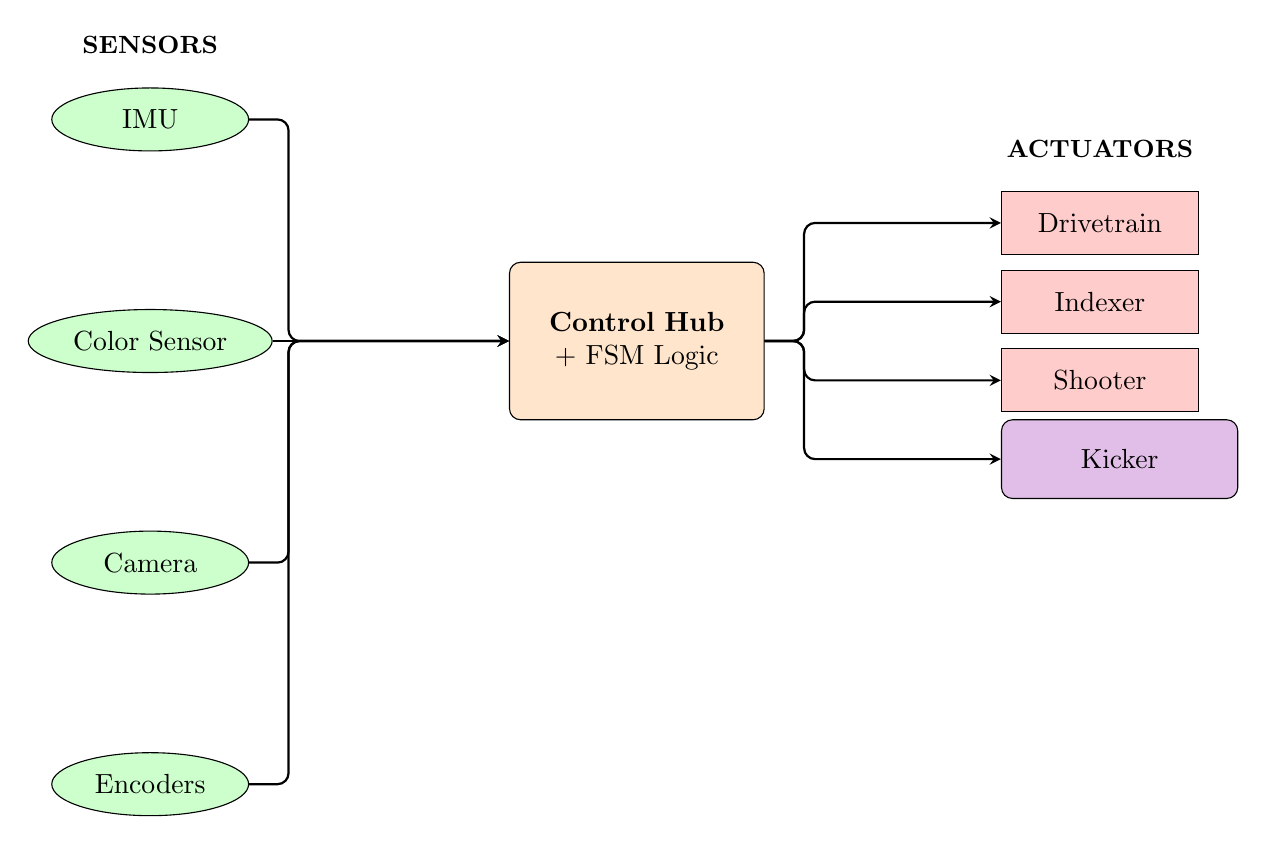
\begin{tikzpicture}[node distance=2cm, auto]

% Sensors (inputs) - left side
\node (imu) [sensor] {IMU};
\node (color) [sensor, below=of imu] {Color Sensor};
\node (camera) [sensor, below=of color] {Camera};
\node (encoders) [sensor, below=of camera] {Encoders};

% Controller - center
\node (hub) [hardware, right=3cm of color, text width=3cm, minimum height=2cm] {\textbf{Control Hub}\\+ FSM Logic};

% Outputs - right side
\node (drive) [motor, right=3cm of hub, yshift=1.5cm] {Drivetrain};
\node (indexer) [motor, right=3cm of hub, yshift=0.5cm] {Indexer};
\node (shooter) [motor, right=3cm of hub, yshift=-0.5cm] {Shooter};
\node (kicker) [action, right=3cm of hub, yshift=-1.5cm] {Kicker};

% Arrows - inputs to hub
\draw [arrow] (imu.east) -- ++(0.5,0) |- (hub.west);
\draw [arrow] (color) -- (hub);
\draw [arrow] (camera.east) -- ++(0.5,0) |- (hub.west);
\draw [arrow] (encoders.east) -- ++(0.5,0) |- (hub.west);

% Arrows - hub to outputs
\draw [arrow] (hub.east) -- ++(0.5,0) |- (drive.west);
\draw [arrow] (hub.east) -- ++(0.5,0) |- (indexer.west);
\draw [arrow] (hub.east) -- ++(0.5,0) |- (shooter.west);
\draw [arrow] (hub.east) -- ++(0.5,0) |- (kicker.west);

% Labels
\node[above=0.3cm of imu, font=\small\bfseries] {SENSORS};
\node[above=0.3cm of drive, font=\small\bfseries] {ACTUATORS};

\end{tikzpicture}
\end{center}

\subsection{How Everything Works Together}

\begin{enumerate}
    \item \textbf{Sensors provide input:} IMU gives heading, color sensor detects balls, camera sees AprilTags
    
    \item \textbf{Control Hub processes:} Runs our Java code, executes state machine logic
    
    \item \textbf{State machine decides:} Based on current state and sensor input, determines next action
    
    \item \textbf{Actuators execute:} Motors move robot, indexer rotates, shooter fires, kicker ejects
    
    \item \textbf{Loop repeats:} Every ~20ms (50 Hz), the cycle runs again
\end{enumerate}

\newpage
% ============================================================================
\section{Quick Reference}
% ============================================================================

\subsection{Common Code Patterns}

\begin{lstlisting}[caption={Edge Detection Pattern (Button Press)}]
// Only trigger on button press, not hold
if (gamepad1.cross && !lastCross) {
    // Action happens once per press
    doSomething();
}
lastCross = gamepad1.cross;  // Remember state
\end{lstlisting}

\begin{lstlisting}[caption={Timer Pattern}]
// Start timer
long startTime = System.currentTimeMillis();

// Check elapsed time
long elapsed = System.currentTimeMillis() - startTime;
if (elapsed > 1000) {  // 1 second passed
    // Do next step
}
\end{lstlisting}

\begin{lstlisting}[caption={Motor Position Control}]
// Set target position
motor.setTargetPosition(targetTicks);
motor.setMode(DcMotor.RunMode.RUN_TO_POSITION);
motor.setPower(0.5);

// Check if arrived
if (Math.abs(motor.getCurrentPosition() - targetTicks) < 10) {
    // At target!
}
\end{lstlisting}

\subsection{Important Files}

\begin{center}
\begin{tabular}{|l|l|}
\hline
\textbf{File} & \textbf{Purpose} \\
\hline
\texttt{A1.java} & Basic manual TeleOp \\
\texttt{A3.java} & Smart auto-indexing TeleOp \\
\texttt{DecodeShootingAuto.java} & Full autonomous \\
\texttt{RevolverSubsystem.java} & Ball handling state machine \\
\texttt{SimpleRevolver.java} & Simplified ball handling \\
\texttt{AprilTagNavigator.java} & Vision processing \\
\texttt{MecanumDrive.java} & Road Runner drivetrain \\
\hline
\end{tabular}
\end{center}

\end{document}
